%% Manuscript for submission to SIAM 
\documentclass[final,leqno,]{siamltex1213}
% options that require additional .clo file:  
% onetabnum: to number equations consecutively with a single digit, instead of using the section number
% onetabnum: numbers tables consecutively throughout the paper
% onefignum: numbers figures consecutively throughout the paper

\usepackage[text={6in,8in},centering]{geometry} % load first
\usepackage{amsmath}
\usepackage{graphicx}
\usepackage{subfig}
\usepackage{textcomp}
\usepackage{xspace}

\graphicspath{{figs/}} %  PATH to figure files-- change to ./ for submission

% CUSTOM COMMAND DEFINITIONS
\newcommand{\R}{\mathbb{R}}
\newcommand{\Z}{\mathbb{Z}}
\newcommand{\K}{\mathbb{K}}
\newcommand{\cpu}{\textsc{cpu}}
\newcommand{\gpu}{\textsc{gpu}}

\newcommand{\bem}{\textsc{bem}\xspace}
\newcommand{\fmm}{\textsc{fmm}\xspace}
\newcommand{\fmmbem}{\fmm-\bem}

\newcommand{\cpp}{\textsc{c++}}
\newcommand{\blas}{\textsc{blas}}
\newcommand{\sse}{\textsc{sse}}

% CURLY LETTERS
\newcommand{\bigO}{\mathcal{O}}
\renewcommand{\O}[1]{\mathcal{O}(#1)}

% FMM OPERATOR DEFINITIONS
\newcommand{\ptom}{\textsc{p}\texttwooldstyle\textsc{m}\xspace} % P2M
\newcommand{\ltop}{\textsc{l}\texttwooldstyle\textsc{p}\xspace} % L2P
\newcommand{\mtop}{\textsc{m}\texttwooldstyle\textsc{p}\xspace} % M2P
\newcommand{\mtom}{\textsc{m}\texttwooldstyle\textsc{m}\xspace} % M2M
\newcommand{\mtol}{\textsc{m}\texttwooldstyle\textsc{l}\xspace} % M2L
\newcommand{\ltol}{\textsc{l}\texttwooldstyle\textsc{l}\xspace}  % L2L
\newcommand{\ptop}{\textsc{p}\texttwooldstyle\textsc{p}\xspace} % P2P

% MISC THINGS
\newcommand{\ncrit}{N_{\text{CRIT}}}
\newcommand{\pmin}{p_{\text{min}}}
\newcommand{\tsolve}{t_{\text{solve}}}


% SOLVER DEFINITIONS
\newcommand{\cg}{\textsc{cg}}
\newcommand{\gmres}{\textsc{gmres}\xspace}
\newcommand{\fgmres}{\textsc{fgmres}\xspace}
\newcommand{\bicgstab}{\textsc{bicgstab}\xspace}

% the text 'd' for integrals
\newcommand{\di}[1]{\text{d}#1}
% partial derivatives (frac)
\newcommand{\partiald}[2]{\frac{\partial #1}{\partial #2}}
% partial derivatives (inline)
\newcommand{\partialdi}[2]{\partial #1 / \partial #2}
% \hat{n}
\newcommand{\nhat}{\hat{n}}
% define a vector - undertilde
%\newcommand{\vect}[1]{\utilde{#1}}
% - bold
\newcommand{\vect}[1]{\mathbf{#1}}
% curly L
\renewcommand{\L}{\mathcal{L}}
% curly D
\newcommand{\D}{\mathcal{D}}
% sign
\newcommand{\sign}{\text{sign}}
% basis vectors
\newcommand{\e}{\vect{e}}
% dyadic product
\newcommand{\dyad}[2]{#1 \otimes #2}







\title{INEXACT KRYLOV ITERATIONS AND RELAXATION STRATEGIES WITH FAST-MULTIPOLE BOUNDARY ELEMENT METHOD} 

\author{Lorena A. Barba\thanks{The George Washington University, Washington DC, 20056 
(\email{labarba@gwu.edu})}
\and Simon K. Layton\thanks{If you want to be first author, you have to write ...}}



\begin{document}
\maketitle
%\slugger{sisc}{xxxx}{xx}{x}{x--x}
%slugger should be set to mms, siap, sicomp, sicon, sidma, sima, simax, sinum, siopt, sisc, or sirev

\begin{abstract}
Abstract text here.
\end{abstract}

\begin{keywords}\end{keywords}

\begin{AMS}\end{AMS}


\pagestyle{myheadings}
\thispagestyle{plain}
\markboth{L. A. Barba and S. K. Layton}{INEXACT KRYLOV ITERATIONS AND RELAXATION STRATEGIES}

\section{Introduction}

Lorem ipsum ...


%% METHODS
\section{Methods for the integral solution of elliptic equations using inexact {\small GMRES}}

\subsection{Boundary-integral solution of the Laplace equation}

To write the Laplace equation, $\nabla^{2}\phi(\vect{x}) = 0$,  in its integral formulation, we use the classical procedure of multiplying by the Green's function and integrating, applying the divergence theorem of Gauss and the chain rule, then dealing with singularities by a limiting process. This results in
%
\begin{equation}\label{eqn:laplace_bem_final}
	\frac{1}{2}\phi + \int_{\Gamma} \phi\partiald{G}{\nhat}\;\di{\Gamma} = \int_{\Gamma}\partiald{\phi}{\nhat}G\;\di{\Gamma},
\end{equation}

\noindent where $G = 1/4\pi r$ is the free-space Green's function for the Laplace equation ($\nabla^{2}G = -\delta$),  $\partiald{\cdots}{\nhat}$ represents the partial derivative in the direction normal to the boundary surface, and the integrals are on the boundary $\Gamma$ of the domain. The boundary element method consists of discretizing the boundary into surface panels and enforcing Equation \eqref{eqn:laplace_bem_final} on a set of target points (collocation version). In its typical form, surface panels take a constant value $\phi_j$, and the surface integrals become sums over $N$ flat surface elements, $\Gamma_j$, resulting in the following discretized equation:
%
\begin{equation}
	\frac{1}{2}\phi_i = \sum_j^{N} \partiald{\phi_j}{\nhat_j}\;\int_{\Gamma}G_{ij}\di{\Gamma_j} - \sum_j^{N} \phi_j\int_{\Gamma}\partiald{G_{ij}}{\nhat_j}\;\di{\Gamma_j}.
\end{equation}

Either the values of the potential or its normal derivative on each panel could be known from boundary conditions, resulting in either first-kind or second-kind integral equations. Finding the remaining unknowns requires solving a system of linear equations $A\vect{x}=\vect{b}$, where the elements of the coefficient matrix are
%
\begin{equation}
	A_{ij} = 
	\begin{cases}
		\int_{\Gamma} G_{ij}\;\di{\Gamma_j}, & \phi\;\text{given on panel}\;j \\
		\int_{\Gamma} \partiald{G_{ij}}{\nhat_j}\;\di{\Gamma_j}, & \partiald{\phi}{\nhat}\;\text{given on panel } j
	\end{cases}
\end{equation}

\noindent
and $\vect{b}$ is formed with the known terms: e.g., if $\phi$ is given on panel $j$, then $\phi_j\int_{\Gamma_j}\partialdi{G_{ij}}{\nhat_j}\;\di{\Gamma_j}$ will appear in the term $b_i$ on the right-hand side of the linear system.

Inserting for $G_{ij}$ and $\partialdi{G_ij}{\nhat_j}$ in terms of $1/r$ and $\nhat_j\cdot\nabla(1/r)$ results in
%
\begin{eqnarray}
	\label{eqn:laplace_bem_G}\int_{\Gamma} G_{ij}\;\di{\Gamma_j} & = & \int_{\Gamma} \frac{1}{|\vect{x}_i-\vect{x}_j|} \;\di{\Gamma_j} \\ 
	\label{eqn:laplace_bem_dGdn}\int_{\Gamma} \partiald{G_{ij}}{\nhat_j}\;\di{\Gamma_j} & = & \int_{\Gamma}\frac{d\vect{x}\cdot\nhat_j}{|\vect{x}_i-\vect{x}_j|^{3}}\;\di{\Gamma_j}
\end{eqnarray}

The next step is to apply an appropriate numerical integration scheme in order to generate all the terms of the coefficient matrix.

\subsection{Boundary-integral solution of the Stokes equation}

\subsection{Numerical integration methods}

\subsection{Krylov subspace methods}

\subsection{Fast multipole method}

%$ RESULTS
\section{Results and discussion}

\subsection{Inexact {\small GMRES} for the solution of Laplace's equation}
To start, we looked at grid-convergence comparing with the analytical solution using a sphere with constant potential and charge on the surface: $\phi = \partialdi{\phi}{\nhat} = 1$. To make surface triangulations of a sphere with increasing refinement, we started with an 8-triangle closed surface, then split recursively each triangle into four smaller ones. Figure \ref{fig:glob_spheres} shows two example discretizations. We solved the boundary-element problem by collocation in both the first-kind and second-kind integral formulations, using a standard right-preconditioned \gmres with fast-multipole-accelerated matrix-vector products and the semi-analytical integrals for the singular terms. For the far-field approximations, we used spherical-harmonic expansions with the following parameters in the \fmm: $\theta_{\text{MAC}} = 0.5$, $p = 10$, and a tolerance of $10^{-6}$ in the iterative solver. 
Figure \ref{fig:laplaceconvergence} shows the resulting convergence for both first-kind and second-kind formulations of the boundary element method on a sphere. They display the expected orders of convergence for boundary element methods: slightly faster than $\O{1/\sqrt{N}}$ in the 1st-kind formulation and $\O{1/N}$ for the 2nd-kind formulation. This gives confidence on our \bem code, the singular/near-singular integral calculations, and the far-field approximation using the \fmm.




\begin{figure}[h]
\begin{center}
	\subfloat[][128 panels]{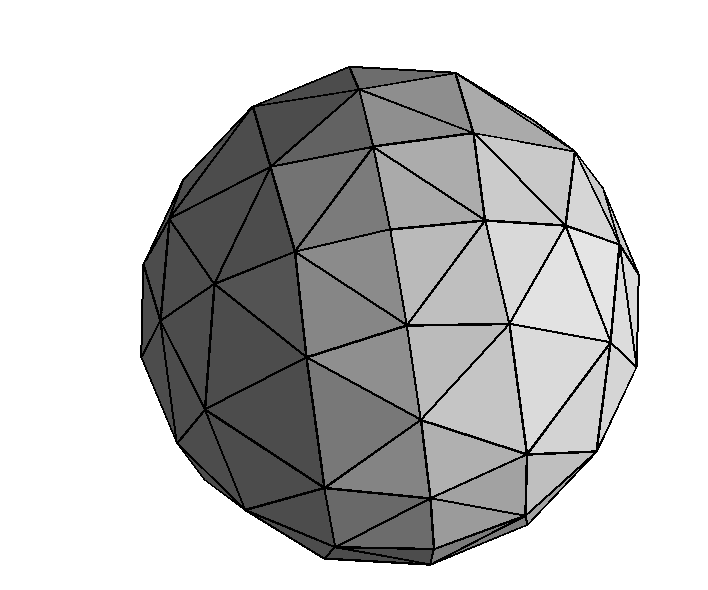
\includegraphics[natwidth=4.73in,natheight=3.94in,width=0.4\textwidth]{sphere128.pdf}\label{fig:sphere128}}\qquad
	\subfloat[][2048 panels]{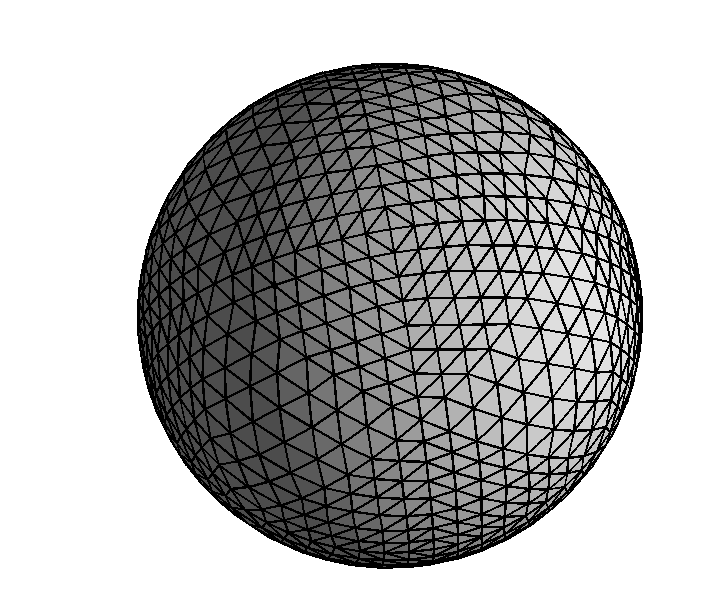
\includegraphics[natwidth=4.73in,natheight=3.94in,width=0.4\textwidth]{sphere2048.pdf}\label{fig:sphere2048}}
	\caption{Triangular discretizations of a spherical surface.}
	\label{fig:glob_spheres}
\end{center}
\end{figure}
%
\begin{figure}[t]
\begin{center}
	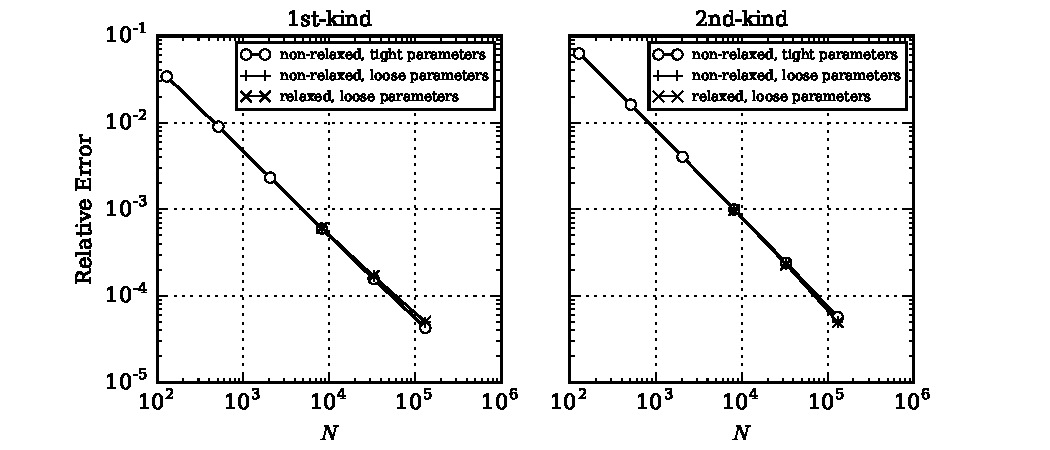
\includegraphics[natwidth=3in,natheight=2in,width=0.5\textwidth]{LaplaceConvergence.pdf}
	\caption{Convergence of 1st-kind (open circles with solid line) and 2nd-kind (open circles with dotted line) solvers for the Laplace equation on a sphere, using a right-preconditioned \gmres with \fmm-accelerated matrix-vecctor products, with parameters: $\theta_{\text{MAC}} = 0.5$, $p=10$, and solver tolerance of $10^{-6}$ (no relaxation).}
	\label{fig:laplaceconvergence}
\end{center}
\end{figure}

Next, we looked at the following test to see how the residual changes as the \gmres iterations proceed and  what value of $p$ is required in the \fmm-accelerated mat-vecs to continue convergence. We discretized a sphere with $32,768$ surface triangles and solved a first-kind integral equation using a solver tolerance of $10^{-5}$ with an initial value of $p$ set to 8. As the residual gets smaller, the value of $p$ needed to maintain convergence of the solver drops, and a low-$p$ of just 3 is sufficient by the seventh iteration. This offers the potential for substantial speed-ups in the calculations, because the translation operators of the \fmm scale from $\bigO(p^{4})$ for spherical harmonics to $\bigO(p^{6})$ for Cartesian expansions.
But we note that only the far-field evaluation can be sped-up with the relaxation strategy, which means that the correct balance between near field and far field in the \fmm could change as we reset $p$ in the later iterations.

\begin{figure}[h]
	\centering
	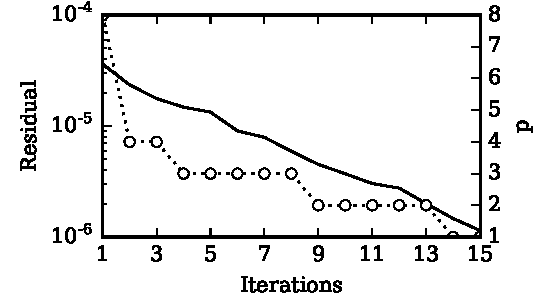
\includegraphics[natwidth=3.7in,natheight=2in,width=0.65\textwidth]{LaplaceResidualIterations.pdf}
	\caption{In a test using a sphere discretized with $32,768$ triangles, the residual $\|r_{k}\|$  (solid line, left axis) decreases with successive \gmres iterations while the necessary $p$ (open circles, right axis) to achieve convergence drops quickly.}
	\label{fig:residualp}
\end{figure}

To find out how much is the potential speed-up, we compared the time to solution for different cases with and without the relaxation strategy. Using three surface discretizations, we solved the boundary-element problem with 1st- and 2nd-kind formulations to a solver tolerance of $10^{-5}$, using a multi-threaded evaluator on 4 \cpu\ cores. In each case, we were careful to set the value of $\ncrit$ to minimize the time to solution of the particular test case. Figure \ref{fig:relaxation_timing} shows the speed-up in the time spent solving the linear system of equations to the specified tolerance. The detailed results are given in the subsequent Tables.


\begin{figure}%[h]
	\centering
	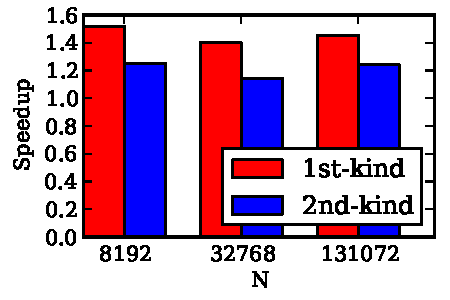
\includegraphics[natwidth=3in,natheight=2in,width=0.45\textwidth]{LaplaceSpeedupRelaxation.pdf}
	\caption{Speedup using a relaxation strategy for three different triangulations of a sphere, using 1st-kind and 2nd-kind integral formulations. (Multi-threaded evaluator running on 4 \cpu\ cores.)}
	\label{fig:relaxation_timing}
\end{figure}


\begin{table}[h]
\footnotesize
\begin{center}
\begin{tabular}{c|cc|cc|c}
  & \multicolumn{2}{c|}{Non-Relaxed} & \multicolumn{2}{c|}{Relaxed} & \\
  N & $\ncrit$ & $\tsolve$ & $\ncrit$ & $\tsolve$ & Speed-up \\
 \hline
   & & & & & \\
  2048 & 400 & 0.27 & 200 & 0.40 & 0.675 \\
  8192 & 400 & 2.58 & 200 & 1.7 & 1.52 \\
  32768  & 400 & 7.1 & 200 & 5.07 & 1.40 \\
  131072  & 400 & 30.1 & 200 & 20.72 & 1.45 \\
 
\end{tabular}
\end{center}
\caption{Speed-ups for the relaxation strategy on a Laplace 1st-kind integral solver, $p=8$, solver tolerance $10^{-5}$.}
\label{tab:laplace_1st_relaxation}
\end{table}%

\begin{table}[h]
\footnotesize
\begin{center}
\begin{tabular}{c|cc|cc|c}
  & \multicolumn{2}{c|}{Non-Relaxed} & \multicolumn{2}{c|}{Relaxed} & \\
  N & $\ncrit$ & $\tsolve$ & $\ncrit$ & $\tsolve$ & Speed-up \\
 \hline
   & & & & & \\
  2048 & 400 & 0.13 & 200 & 0.64 & 0.20 \\
  8192 & 400 & 1.49 & 200 & 1.19 & 1.25 \\
  32768 & 400 & 6.77 & 200 & 5.92 & 1.14 \\
  131072 & 400 & 30.01 & 200 & 24.2 & 1.24 \\
 
\end{tabular}
\end{center}
\caption{Speed-ups for the relaxation strategy on a Laplace 2nd-kind integral solver, $p=8$, solver tolerance  $10^{-5}$.}
\label{tab:laplace_2nd_relaxation}
\end{table}%

The results on Tables \ref{tab:laplace_1st_relaxation} and \ref{tab:laplace_2nd_relaxation} show a speed-up for the three larger grids---also plotted on Figure \ref{fig:relaxation_timing}---of about $1.4\times$ for the 1st-kind integral formulation and $1.2\times$ for the 2nd-kind formulation. These are moderate speedups, but these tests already taught us something: that one has to give up on the idea of partitioning the domain between a near-field and a far-field in a way that balances the time spent computing each one---an accepted idea in \fmm applications. When relaxing the accuracy of the \gmres iterations, the time taken to compute the far field decreases significantly. This means that to minimize time-to-solution when using relaxed \gmres, the near and far fields should not be balanced, but rather the far field should be bloated. As a result, the first couple of iterations are completely dominated by the time to compute the far field, but this is offset by the benefit of much cheaper iterations from then on. This is a simple but unexpected and counter-intuitive algorithmic consequence of the idea of inexact \gmres with \fmm.

It's clear that greater benefits from the relaxation strategy should derive from two situations: (a) where higher accuracy is needed (necessitating an initially higher $p$) , and (b) where the linear system demands a greater number of iterations to reach a set tolerance (resulting in more computations done at low $p$). To demonstrate this, we now present two tests that force these situations. 

\begin{figure}[h]
	\centering
	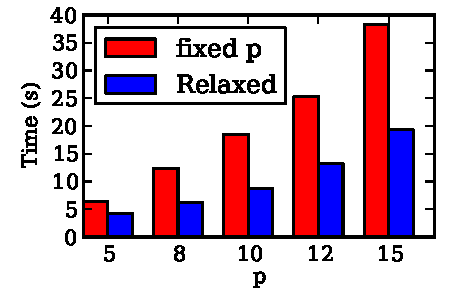
\includegraphics[natwidth=3in,natheight=2in,width=0.45\textwidth]{LaplaceRelaxationP.pdf}
	\caption{Timings for solving a 1st-kind Laplace integral formulation on a sphere discretized with $32,768$ panels, using a relaxed \gmres with different initial values of $p$, compared with a fixed-$p$ solver. The iteration count was capped at 10 for all cases. (Multi-threaded evaluator running on 4 \cpu\ cores.)}
	\label{fig:laplace_p_speedup}
\end{figure}

Figure \ref{fig:laplace_p_speedup} shows the timings obtained in a situation where the initial $p$ is incrementally larger, representing applications that demand higher accuracy. The test consists of a 1st-kind Laplace integral solver on a sphere discretized with $32,768$ panels, enforcing a fixed number of $10$ \gmres iterations (which results in a residual of $~5.5\times 10^{-5}$ for the sphere). Table \ref{tab:laplace_1st_p_relaxation} shows the data for this test: the speed-up is greater with larger initial values of $p$, leveling at around $2\times$ when initial $p$ is greater than 8. Note again that the shortest time-to-solution requires an unbalanced tree on the first iteration, with a bloated far field. This means that the first (high-$p$) iteration is much slower than the corresponding fixed-$p$ case: the speed-up is thus purely a product of the low-cost later iterations.

\begin{table}[h]
\footnotesize
\begin{center}
\begin{tabular}{c|cc|cc|c}
  & \multicolumn{2}{c|}{Relaxed} & \multicolumn{2}{c|}{Non-Relaxed} & \\
  $p$ & $\ncrit$ & $\tsolve$ & $\ncrit$ & $\tsolve$ & Speedup \\
   \hline
   & & & & & \\
  5 & 100 & 4.21 & 100 & 6.34 & 1.51 \\
  8 & 100 & 6.24 & 400 & 12.4 & 1.99 \\
  10 & 150 & 8.76 & 400 & 18.5 & 2.11 \\
  12 & 150 & 13.2  & 600 & 25.3 & 1.92 \\
  15 & 150 & 19.3 & 600 & 38.3 & 1.98 \\
 
\end{tabular}
\end{center}
\caption{Speed-up when using a relaxation strategy on a Laplace 1st-kind integral solver, compared with a non-relaxed solver, with increasing value of the initial $p$ (representing increased accuracy demands of the application), for a sphere discretized with $32,768$ panels. (Multi-threaded evaluator running on 4 \cpu\ cores.)}
\label{tab:laplace_1st_p_relaxation}
\end{table}%

The final case looks at the situation where the application might demand large iteration counts, as could be encountered in harder-to-precondition cases. Keeping the value of $p$ fixed at 10, we ran several cases with increasing number of (set) \gmres iterations, representing more ill-conditioned problems. Figure \ref{fig:laplace_iterations_speedup} shows how cases with larger iteration counts experience greater speed-up from the relaxation strategy. As seen in the data of Table \ref{tab:laplace_1st_iterations_relaxation}, each non-relaxed iteration adds approximately $1.68$s to $\tsolve$, while each relaxed iteration adds $0.276$s; we can thus extrapolate a speed-up nearing $5\times$ at 100 iterations.



\begin{figure}[h]
	\centering
	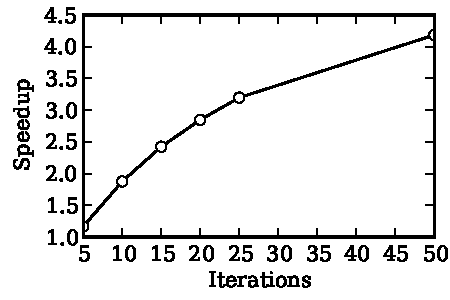
\includegraphics[natwidth=3in,natheight=2in,width=0.5\textwidth]{LaplaceRelationIterations.pdf}
	\caption{Speed-ups for solving a 1st-kind Laplace integral problem on a sphere discretized with $32,768$ panels, as the \gmres iteration count increases; $p=10$ for all cases. (Multi-threaded evaluator running on 4 \cpu\ cores.)}
	\label{fig:laplace_iterations_speedup}
\end{figure}


\begin{table}[h]
\footnotesize
\begin{center}
\begin{tabular}{c|cc|cc|c}
  & \multicolumn{2}{c|}{Relaxed} & \multicolumn{2}{c|}{Non-Relaxed} & \\
  Iterations & $\ncrit$ & $\tsolve$ & $\ncrit$ & $\tsolve$ & Speedup \\
 \hline
   & & & & & \\
  5 & 100 & 8.57 & 400 & 10.0 & 1.17 \\
  10 & 100 & 9.81 & 400 & 18.4 & 1.88 \\
  15 & 100 & 11.1 & 400 & 26.9 & 2.42 \\
  20 & 100 & 12.4 & 400 & 35.3 & 2.85 \\
  25 & 100 & 13.7 & 400 & 43.8 & 3.20 \\
  50 & 100 & 20.6 & 400 & 86.2 & 4.18 \\
 
\end{tabular}
\end{center}
\caption{Speed-up of the relaxation strategy on solving a Laplace 1st-kind integral problem on a sphere discretized with $32,768$ panels, with increasing iteration count; $p$ fixed to a value of 10. (Multi-threaded evaluator running on 4 \cpu\ cores.)}
\label{tab:laplace_1st_iterations_relaxation}
\end{table}%

\subsection{Inexact {\small GMRES} for solving the Stokes equation}
Like before, we start with a grid-convergence study to build confidence that the Stokes solver is correct and converges to the right solution at the expected rate. As an application of the Stokes equation, we chose low-Reynolds-number flow, using a spherical geometry for the grid-convergence study. This classical problem of fluid mechanics has an analytical solution that gives the drag force on the sphere as $F_d = 6\pi\mu Ru_x$, where $\mu$ is the viscosity of the fluid, $R$ is the Reynolds number and $u_x$ is the free stream velocity, taken in the $x$-direction. We solve a first-kind integral equation for the traction force, $\vect{t}$, by imposing $\vect{u} = (1,0,0)^{T}$ at the center of every panel, and compute the drag force with

\begin{equation}
	\label{eqn:stokes_traction_drag}
	F_d = \int_\Gamma t_x\;\di{\Gamma'} = \sum_{j=1}^{N} t_{x_j}\cdot A_j
\end{equation}

For all the tests, we set $R=1$, $u_x = 1$ and $\mu = 10^{-3}$, giving a drag force of $F_d = 0.01885$. We solve the integral problem using a boundary element method with fast-multipole-accelerated mat-vecs in a \gmres solver. We first increased the value of $p$ until the solution stopped improving, and settle for $p=16$ in this case, using a $10^{-5}$ tolerance in the iterative solver.
Figure \ref{fig:stokes_convergence} shows that we indeed observe convergence at the expected rate of $\O{1 / \sqrt{N}}$, for first-kind integral equations.

\begin{figure}[h]
\begin{center}
	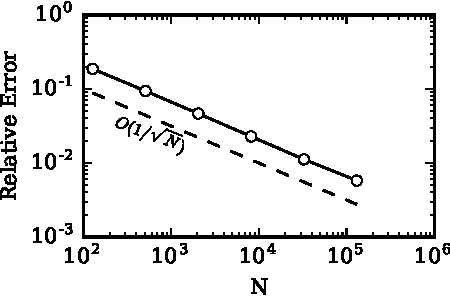
\includegraphics[natwidth=3in,natheight=2in,width=0.5\textwidth]{StokesConvergence.pdf}
	\caption{Convergence of first-kind equation for Stokes flow around a sphere. Initial $p=16$, linear system solved to $10^{-5}$ tolerance.}
	\label{fig:stokes_convergence}
\end{center}
\end{figure}

Like with the Laplace equation, we need to show that the relaxation strategy does not hinder convergence and that there is a potential for speed-ups. We solved the problem of Stokes flow around a sphere, discretized with $8,192$ panels, and compared the residual history of a fixed-$p$ solver with a relaxed \gmres with an initial $p=16$. Figure \ref{fig:stokes_residual_history_relaxed} shows that the residual history (for the traction force) is similar for both relaxed and non-relaxed \gmres, both methods reaching the stipulated tolerance of $10^{-5}$ after about 27 iterations.
The number of iterations needed to converge is larger in the case of the Stokes equation compared to the Laplace equation, which bodes well for the speed-up that we could get from relaxation. Moreover, the fast multipole expansions for the Stokes kernel are equivalent to four Laplace expansions, which combines with the larger number of iterations to offer greater speed-ups.


\begin{figure}[h]
\begin{center}
	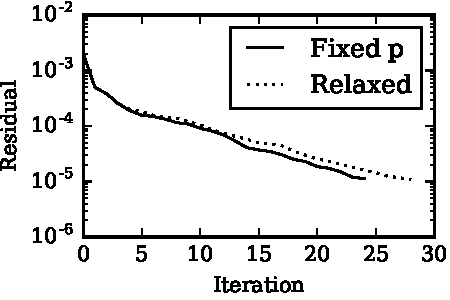
\includegraphics[natwidth=3in,natheight=2in,width=0.5\textwidth]{StokesResidualHistory.pdf}
	\caption{Residual history solving for surface traction on the surface of a sphere (first-kind integral problem), with a $10^{-5}$ solver tolerance, $8,192$ panels, and $p=16$ in the multipole expansions.}
	\label{fig:stokes_residual_history_relaxed}
\end{center}
\end{figure}

Figure \ref{fig:stokes_relaxation_breakdown} illustrates clearly how we need to adjust the balance between near field and far field when using relaxation strategies. Because most of the time is spent computing at the low values of $p$, we need to start with a bloated far field. The bar plot shows the breakdown of time spent in the {\ptop} and {\mtol} kernels for each iteration: although the first iteration is unbalanced, with far field taking about 8 times as much \cpu\ time as near field, later iterations are close to balanced and the total time to solution is optimal. 
The figure also includes a plot of the residual history. We should add that we ran extensive tests on the minimum value of $p$ that could be allowed in the relaxed solver, without degrading convergence and accuracy. Table \ref{tab:stokes_min_p} presents some of the data from these tests: for finer surface discretizations, the error degrades when the relaxed value of $p$ is allowed to drop below 3 or 4. To be conservative and avoid any degradation in accuracy, we used a $\pmin=5$ for all further cases with the Stokes equation.


\begin{figure}[h]
\begin{center}
	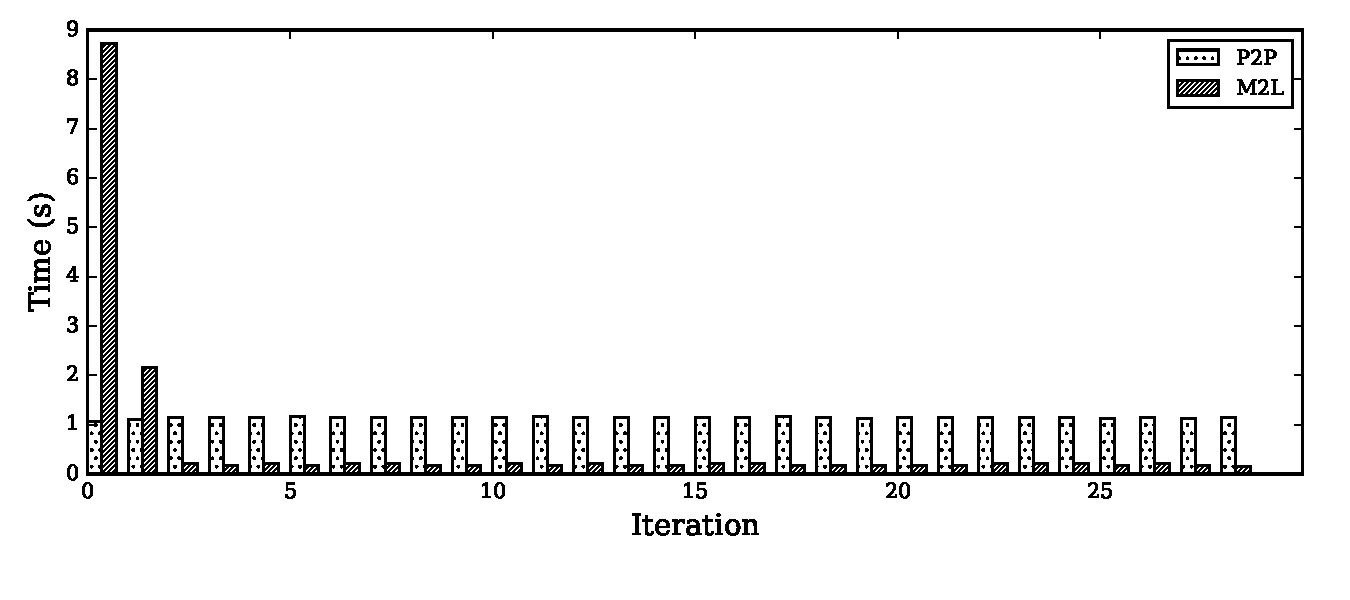
\includegraphics[natwidth=3in,natheight=2in,width=0.5\textwidth]{StokesSolveBreakdown.pdf}
	\caption{Residual history solving for surface traction on the surface of a sphere, with time breakdown between {\ptop} and {\mtol}. $10^{-5}$ solver tolerance, $8,192$ panels, $p=16$.}
	\label{fig:stokes_relaxation_breakdown}
\end{center}
\end{figure}



\begin{table}[ht]
\footnotesize
\begin{center}
\begin{tabular}{c|cc|cc|cc}
  & \multicolumn{2}{c|}{2048 panels} & \multicolumn{2}{c|}{8192 panels} & \multicolumn{2}{c}{32768 panels} \\
 $\pmin$ & Error & $it$ & Error & $it$ & Error & $it$ \\ \hline
  & & & & & & \\
 5 & $4.70\times 10^{-2}$ & 22 & $2.44\times 10^{-2}$ & 28 & $1.34\times 10^{-2}$ & 28 \\
 4 & $4.49\times 10^{-2}$ & 23 & $2.51\times 10^{-2}$ & 29 & $1.25\times 10^{-2}$ & 29 \\
 3 & $4.64\times 10^{-2}$ & 22 & $2.78\times 10^{-2}$ & 29 & $1.39\times 10^{-2}$ & 29 \\
 2 & $4.95\times 10^{-2}$ & 25 & $2.62\times 10^{-2}$ & 33 & $3.18\times 10^{-2}$ & 39 \\
 1 & $4.96\times 10^{-2}$ & 25 & $2.99\times 10^{-2}$ & 51 & $4.77\times 10^{-2}$ & 53 
\end{tabular}
\end{center}
\caption{Effect of $p_{\text{min}}$ on accuracy and convergence for Stokes flow around a sphere for differing values of $N$. Error is on the total drag force in the $x$-direction, $F_x$.}
\label{tab:stokes_min_p}
\end{table}%

Figure \ref{fig:stokes_speedup} shows the speed-up resulting from the relaxed \gmres iterations for four, increasingly finer surface discretizations. For $N=8,192$ and above, speed-up is $3.5\times$ or more.


\begin{figure}[h]
\begin{center}
	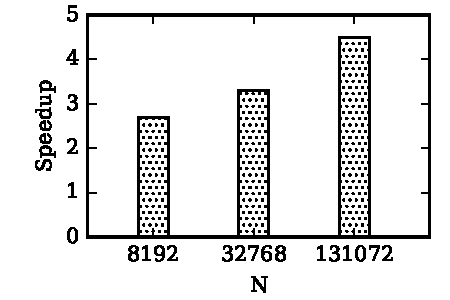
\includegraphics[natwidth=3in,natheight=2in,width=0.5\textwidth]{StokesSpeedupRelaxation.pdf}
	\caption{Speed-up for solving first-kind Stokes equation on the surface of a sphere, varying $N$. $10^{-5}$ solver tolerance, $p=16$. }
	\label{fig:stokes_speedup}
\end{center}
\end{figure}

\subsection{Application to red blood cells in Stokes flow}

A number of medical applications will benefit from greater understanding of the microflows around red blood cells and of the mechanical effects on the cells from this flow. 
The most notable example is perhaps the deadly malaria infection, which changes red blood cells making them stiffer thus disrupting the flow of blood in capillaries \cite{FedosovETal2011}.
Any design of a biomedical device that processes blood at the micrometer-scale needs to consider the mechanical behavior of blood at the cellular level \cite{Freund2014}. Blood is a dense suspension of mostly red blood cells and smaller concentrations of white blood cells and platelets. The flow regime in small capillaries is at very low Reynolds numbers, and thus completely dominated by viscous effects. 
Red blood cells are very flexible, so any physiologically realistic simulation should take into account their elastic deformations. But here we are only attempting to show the benefit of our relaxation strategy on the Stokes solver, and thus limit our study to the steady Stokes flow around a red-blood-cell geometry. The unsteady problem of coupled Stokes flow and linear elasticity can be approached by repeated solution of boundary-integral problems at every time step, and would equally benefit from the speed-ups seen on a single Stokes solution.

To create a surface discretization for a red blood cell, we start with a sphere discretized into triangular panels and transform every vertex $v = v(x,y,z)$, with $x,y,z\in [-1,1]$, into $v' = v'(x',y',z(\rho'))$ using the formula presented in Ref.~\cite{EvansFung1972}:

\begin{equation}
	\label{eqn:rbc_parameterization}
	z(\rho) = \pm \frac{1}{2}\sqrt{1 - \left(\frac{\rho}{r}\right)^{2}}\left ( C_0 + C_2 \left(\frac{\rho}{r}\right)^{2} + C_4\left(\frac{\rho}{r}\right)^{4}\right )
\end{equation}

\noindent where $x' = x\cdot r,\; y' = y\cdot r,\; \rho = \sqrt{x'^{2}+y'^{2}}$. Table \ref{tab:rbc_parameterization_constants} lists the constants in this equation and  Figure \ref{fig:glob_rbc} shows two examples of transformed shapes obtained from sphere triangulations using Equation \eqref{eqn:rbc_parameterization}.

\begin{table}[t]
\footnotesize
\begin{center}
\begin{tabular}{c|c|c|c}
	$r$ & $C_0$ & $C_2$ & $C_4$ \\   \hline
	& & &\\
	  $3.91\mu$m & $0.81\mu$m  & $7.83\mu$m  & $-4.39\mu$m
\end{tabular}
\end{center}
\caption{Constants for equation \eqref{eqn:rbc_parameterization}, from Ref.~\cite{EvansFung1972}. }
\label{tab:rbc_parameterization_constants}
\end{table}%


\begin{figure}[b]
\begin{center}
	\subfloat[512 panels]{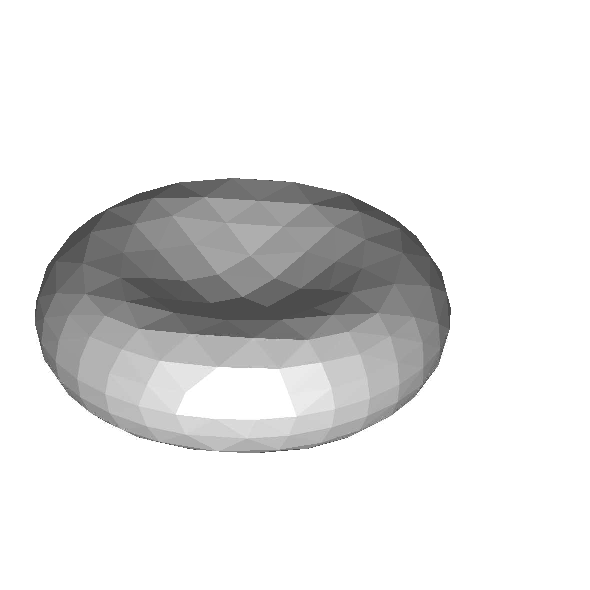
\includegraphics[natwidth=2.94in,natheight=1.94in,width=0.35\textwidth]{RBC512.pdf}\label{fig:rbc512}}\qquad
	\subfloat[2048 panels]{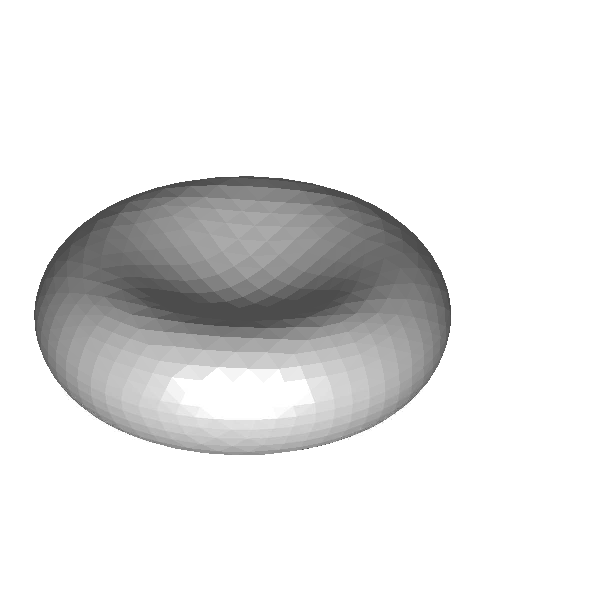
\includegraphics[natwidth=2.94in,natheight=1.94in,width=0.35\textwidth]{RBC2048.pdf}\label{fig:rbc2048}}
	\caption{Surface geometries of red blood cells obtained from transforming sphere triangulations using Equation \eqref{eqn:rbc_parameterization}.}
	\label{fig:glob_rbc}
\end{center}
\end{figure}

A grid-convergence study using the geometry of a red blood cell requires that we use Richardson extrapolation \cite{roache1998}, since we don't have an analytical solution for this situation. We calculated the drag on a red blood cell in uniform Stokes flow using three surface meshes, consecutively refined by a constant factor $c=4$. 
If the value $f_1$ corresponds to that obtained using the coarsest mesh and $f_3$ with the finest, then we can obtain the extrapolated value approximating the exact solution with the following formula:
%
\begin{equation}
	\bar{f} = \frac{f_1f_3-f_2^{2}}{f-1 -2f_2+f_3}
\end{equation}

Table \ref{tab:rbc_richardson_values} presents the computed value of the drag force with three different meshes, of sizes $N=512, 2048$ and $8192$. We can also obtain the \emph{observed order of convergence}, $p$, as follows
%
\begin{equation}
	p = \frac{\ln{\left(\frac{f_2-f_1}{f_3-f_2}\right)}}{\ln{c}},
\end{equation}

\noindent where $c$ is the refinement ratio between two consecutive meshes. With the values in Table \ref{tab:rbc_richardson_values}, we obtain an observed order of convergence of $0.481$, matching our expected rate of convergence of $\O{\sqrt{N}}$. 
Figure \ref{fig:rbc_extrapolated_convergence} shows a plot of the error with respect to the mesh size, using the extrapolated value as a reference.

\begin{table}[h]
\footnotesize
\begin{center}
\begin{tabular}{c|c}
	$N$ & $f_x$ \\
	\hline
	& \\
	$512$ & $-0.059$ \\
	$2048$ & $-0.071$ \\ 
	$8192$ & $-0.077$ \\
%	$32768$ & $-0.080$
\end{tabular}
\end{center}
\caption{Surface mesh sizes and calculated drag force for the convergence study using a red blood cell in uniform Stokes flow.}
\label{tab:rbc_richardson_values}
\end{table}%


\begin{figure}
\begin{center}
	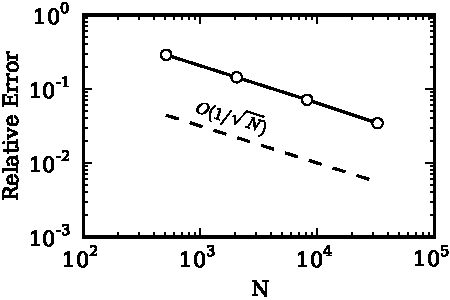
\includegraphics[natwidth=3in,natheight=2in,width=0.5\textwidth]{EthrocyteConvergence.pdf}
	\caption{Observed convergence for Stokes flow around red blood cells, with respect to the extrapolated value of the drag coefficient, using Richardson extrapolation \cite{roache1998}.}
	\label{fig:rbc_extrapolated_convergence}
\end{center}
\end{figure}


%Cited in \cite{kruger2012}

\section{Conclusion} 

We have shown the first successful application of a relaxation strategy for fast-multipole-accelerated boundary element methods, based on the theory of inexact \gmres. Testing the relaxation strategy on Laplace problems, we confirmed that it converges to the right solution, it provides moderate speed-ups over using a fixed $p$, and it leads to initially bloated far-fields to obtain the minimum time to solution.
Exploring the performance advantage of relaxing the value of $p$ as \gmres iterations advance, we concluded that problems requiring high accuracy and/or resulting in more ill-conditioned linear systems will experience the best speed-ups, which for Laplace problems can be in the order of $2-4\times$.

In the case of the Stokes equation, the speed-ups that can be obtained using a relaxation strategy are larger, due to the fact that Stokes problems require both more iterations to converge (and the relaxed solver spends more time at low $p$) and more work per iteration (equivalent to four Laplace evaluations). Relaxed \gmres iterations in this case reduced the time to solution by $3.5\times$ to $4.5\times$. We found that it's important for Stokes problems to also enforce a minimum value of $p$ to avoid accuracy or convergence degradation.


 
%% Acnowledgements

%% Bibliography
\bibliographystyle{siam}
\bibliography{bem,cfd,CompBio,FastMethods,InexactMatVec,scicomp}

\end{document}
%% end of file `docultex.tex'
